\documentclass[a3paper, twoside, openany]{book}
\usepackage[utf8]{inputenc}
\usepackage[T1]{fontenc}
\usepackage[italian]{babel}
\usepackage[normalem]{ulem}
\usepackage{textcomp}
\usepackage{array}
\usepackage{amsmath}
\usepackage{amsfonts}
\usepackage{asymptote}
\usepackage{dirtytalk}
\usepackage{gensymb}
%\usepackage{csquotes}
\usepackage{graphicx}
\graphicspath{{assets/}}
\newenvironment{riq}
    {\begin{center}
    \begin{tabular}{|p{0.9\textwidth}|}
    \hline\vspace{0.5pt}}
    { \vspace{5pt}
    \\\hline
    \end{tabular}
    \end{center}
    }


\title{Studio dei circuiti RC}
\author{Giacomo Fortunato}

\begin{document}
\maketitle
\section{Presentazione}
Mi chiamo \textbf{Giacomo Fortunato} e frequento (ancora per poco) la quinta classe, sezione F, al Liceo Scientifico Statale \say{G. Battaglini}. Questo è il mio elaborato di \textbf{Matematica e Fisica} preparato per la simulazione del colloquio d'esame (a.s. 2019/2020, anche noto come anno del COVID). \\ In questa breve relazione percorreremo le strade matematiche di integrali e limiti per studiare il funzionamento dei circuiti RC (a corrente continua), in particolare il comportamento del \textbf{condensatore}. \\ Questo documento è stato creato utilizzando un linguaggio di markup per la preparazione di testi chiamato \LaTeX\footnote{https://www.latex-project.org/}: questo linguaggio è utilizzato continuamente nella produzione di documenti, tesi, relazioni e pubblicazioni di ogni genere, particolarmente di carattere scientifico. Personalmente, scrivo e compilo (trasformare da file codice a file finale) \LaTeX con Atom\footnote{https://atom.io/}, l'IDE sviluppato da GitHub\footnote{https://github.com/}. Ho appreso di \LaTeX dai miei compagni più grandi delle Olimpiadi di Matematica, e sono fiero di aver imparato così tanto successivamente da solo. \\ Spero che l'elaborato possa essere di Vostro gradimento, buona lettura.
\chapter{Introduzione}
\begin{figure}[htp]
    \centering
    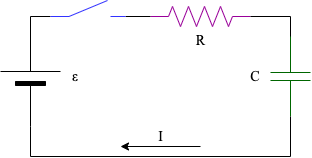
\includegraphics[width=10cm]{Circuito RC-Aperto}
    \caption{Circuito RC aperto}
    \label{fig:RC-aperto}
\end{figure}














\end{document}
